\chapter{Implementation of CN-VIP}\label{chap:impl-cnvip}

\margintoc{}

In addition to designing, formalising, and proving it sound, I also implemented
CN-VIP\@. This was a substantial project which I worked on for about seven
months, from August to October of 2023, and May, June, September and October
of 2024, based on
\href{https://github.com/search?q=repo\%3Arems-project\%2Fcerberus+author\%3Adc-mak\&type=commits\&s=committer-date\&o=asc}{my
commits} to the \kl{Cerberus} repository. In the intervening months, I worked
on a failed update to the \kl{buddy allocator} of pKVM to work with bit-vectors
(\cref{chap:buddy}), engineering for accurate source location information
(\cref{sec:error-msgs}), and MiniCN (\cref{chap:kernel-alternative}).

What made it more challenging was that it had to be developed and integrated
piecemeal alongside other active \kl{CN} development.

The first step was adding in the various pieces of infrastructure in a non-functional way.
\begin{itemize}
    \item A logical variable for allocation history.
    \item A resource predicate for the \cninline{Alloc} token.
    \item Updated rules for \coreinline{create} and \coreinline{kill}, using the \cninline{Alloc} token.
    \item A datatype for the SMT representation of pointers.
    \item A flag to toggle \kl{CN-VIP} features on and off.
    \item Array and member shifting operators.
    \item The \cinline{copy_alloc_id} operator.
\end{itemize}

Given all this, the next steps were about implementing support for bounds and
liveness checks, which was relatively straightforward.
\begin{itemize}
    \item Adapt and categorise the \kl{PNVI}/\kl{VIP} test suite to \kl{CN-VIP}\@.
    \item Support for non-deterministic pointer equality.
    \item Add a pointer liveness check.
    \item Deriving bounds and disjointness constrains.
    \item Basic support for \cinline{memcpy} (no provenance or
        \coreinline{unspec} values).
\end{itemize}

At this stage of development, I switched on CN-VIP by default, but retained the
ability to switch it off behind a flag. Fortunately, this happened just after
benchmarking on the CN tests was added, so we have a measurement of the impact
of the transition, shown in \cref{fig:vip-performance-hit}.

\begin{figure}[h]
    \centering
    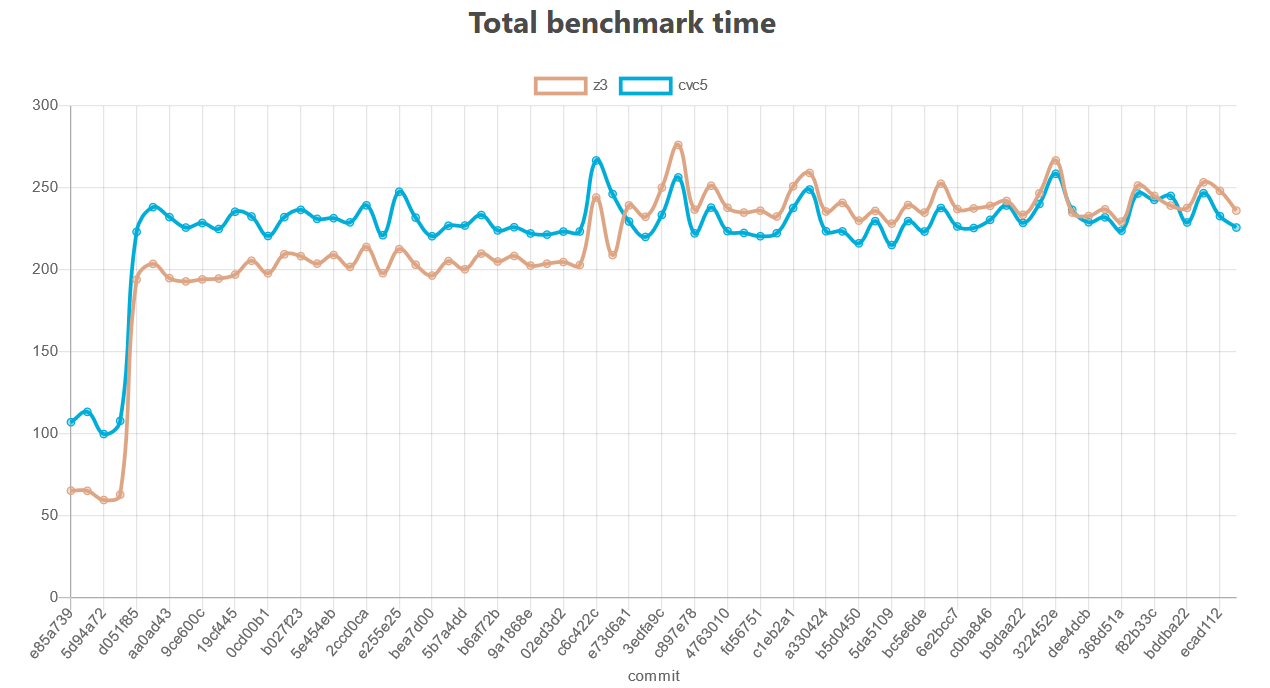
\includegraphics[width=\textwidth]{../misc/vip-performance-hit.png}
    \caption{Sharp increase in execution time when enabling VIP, courtesy of
        \url{https://rems-project.github.io/cn/dev/bench/}.}\label{fig:vip-performance-hit}
\end{figure}

Aside from performance, at this stage, it also became clear that not supporting
provenance in bytes was unworkable \textemdash{} 18 out of 44 tests required
additional \cinline{copy_alloc_id} annotations to work as intended. Lack of
support for round-trip was also an issue, this affected an additional 2 tests.

\begin{itemize}
    \item Support memory bytes.
    \item Support \cinline{memcpy}, \cinline{malloc} and \cinline{free}.
    \item Support comparable bytes for \cinline{memcmp}.
    \item Support round-trip casts.
\end{itemize}

\section{Implementation preliminaries}

\kl{CN} is implemented in OCaml; modifications to extend \kl{Cerberus} to
support \kl{CN} are written in both Lem and OCaml. The output of \kl{Cerberus}
is a \kl{Core} syntax tree, along with annotations and APIs to parse and
resolve symbols in those annotations.

Although \kl{CN} does not A-normalise \kl{Core} any more
(\fancyref{sec:rescore}), it does inline all non-recursive labels, and simplify
the use of C types as values: whereas \kl{Core} supports computing them
dynamically, \kl{CN} requires them to be known statically.\sidenote{The main
limitation this imposes is in supporting indirect calls to functions via
pointers.} The end result of the transformations on \kl{Core} are stored in a
new type called \intro{MuCore}, and it is this type that \kl{CN} type-checks.

There are four types of constructs which \kl{CN} parses, each located in
different places.
\begin{itemize}
    \item \ocamlinline{cn_toplevel}. \kl{CN} logical function, resource predicate,
        and datatype definitions, and \emph{named} function specifications (for
        inclusion in a header file), and placed at the top-level in a C file.
    \item \ocamlinline{cn_statement}. \kl{CN} annotation within function bodies.
        For proof guidance and debugging.
    \item \ocamlinline{function_spec}. \kl{CN} annotations for pre- and
        postconditions, places after a function parameter list but before the
        function body.
    \item \ocamlinline{loop\_spec}. \kl{CN} loop invariants, placed after the loop
        conditions, but before the loop body.
\end{itemize}

The pipeline for obtaining all this is as follows.
\begin{enumerate}
    \item The C program is parsed into a C abstract sytnax tree.
    \item Top-level magic comments are parsed into \ocamlinline{cn_toplevel}s.
    \item Within-function magic statements, function specifications and loop
        specifications are inserted as string annotations on AST nodes.
    \item \kl{Cerberus} desugars the AST (including the \ocamlinline{cn_toplevel}
        constructs), and then elaborates it into Core
    \item \kl{CN} transforms \kl{Core} into \kl{MuCore}, during which process
        the remaining magic comments are parsed and desugared into the same.
\end{enumerate}

After this, the \kl{MuCore } file, specifically all the \kl{CN}-related
declarations, definitions and specifications undergo checks to ensure that they
are well-formed, for example, ensuring that basetypes match.

After that, type-checking is essentially gathering and proving constraints,
querying and manipulating the resource context, and symbolically evaluating
expressions. The type-checker itself is written in a monadic style to
encapsulate all mutable interactions with the constraint context, resource
context, and the SMT solver.

As mentioned in~\fancyref{sec:rescore}, the type-checker is also written in a
continuation-passing style. A continuation awaits the result (a pure/SMT term)
of type-checking the current expression, and uses it to type-check the rest of
the (enclosing) expression. For example, type-checking an if-expression means
duplicating the continuation for each branch, whereas type-checking
undefined-behaviour involves proving false, and then dropping the continuation.

\begin{itemize}
    \item \ocamlinline{Mu}, short for \ocamlinline{Mucore}. Module for the
        \kl{MuCore} syntax tree OCaml type. Contains the type for
        pure expressions, \ocamlinline{'a Mucore.pexpr}, where the type
        parameter is instantiated to \ocamlinline{BaseTypes.t} after
        well-formed checks have been performed.
    \item \ocamlinline{Sym}. Module for resolved symbols. A
        \ocamlinline{SymMap} is \ocamlinline{Sym.t}-indexed map.
    \item \ocamlinline{IntMap}. An integer-indexed map.
    \item \ocamlinline{Id}. Module for identifiers, usually used for members of
        records.
    \item \ocamlinline{BT}, short for \ocamlinline{BaseTypes}. Module for
        basetypes.
    \item \ocamlinline{IT}, short for \ocamlinline{IndexTerms}. Module for
        pure/SMT terms.
    \item \ocamlinline{LC}, short for \ocamlinline{LogicalConstraint}. Module
        for boolean-valued pure/SMT terms which may be quantified with a single
        quantifier.
    \item \ocamlinline{LCSet}. Module for a set of (potentially quantified)
        boolean-valued pure/SMT terms.
    \item \ocamlinline{Global}. Module for storing the definitions of structs,
        datatypes, resource predictates, logical \kl{CN} functions, and
        declarations of C functions and \kl{CN} lemmas.
    \item \ocamlinline{Where}. Module for structuring location information used
        in \kl{CN} error messages.
    \item \ocamlinline{Alloc}. Module defining two submodules,
        \ocamlinline{History} for the allocation history pure/SMT term and associated
        helper functions, and \ocamlinline{Predicate}, for defining the
        allocation token used in the resource context.
    \item \ocamlinline{Definition} Module defining three submodules.
        \begin{itemize}
            \item \ocamlinline{Clause}. Module defining the OCaml type for
                handling the \emph{body} of a resource predicate definition.
            \item \ocamlinline{Predicate}. Module defining the OCaml type for
                handling resource predicate definitions (a list of clauses,
                see~\fancyref{sec:restriction-branching}).
            \item \ocamlinline{Function}. Module defining the OCaml type for
                handling logical \kl{CN} function definitions.
        \end{itemize}
    \item \ocamlinline{Memory}. Module defining helper functions related
        to a choice of the \kl{Cerberus} memory interface, such as the size
        of C types and the layout of structs.
    \item \ocamlinline{SMT}. Module for manipulating SMTLib S-expressions.
    \item \ocamlinline{Locations}. Module for manipulating source locations.
    \item \ocamlinline{CF}, short for \ocamlinline{Cerberus_frontend}. Module
        for helper functions from the \kl{Cerberus}.
    \item \ocamlinline{RI}, short for \ocamlinline{ResourceInference}. Contains
        many modules; its \ocamlinline{Special} module is handles queries for
        (iterated) predicates and checking whether a pointer belongs to a live
        allocation.
    \item \ocamlinline{Typing}. Module for defining the type-checking monad
        \ocamlinline{Typing.m}, which abstracts the details of manipulating the
        typing context as mentioned above.
\end{itemize}

Note that the \ocamlinline{check_pexpr} function, defined in a
continuation-passing style, has type \ocamlinline[breaklines]{BaseTypes.t
Mucore.pexpr -> (IndexTerms.t -> unit Typing.m) -> unit Typing.m}.

\section{Definition of allocation history}

An allocation history is a map from \kl{allocation ID}s (non-empty provenances) to a
record of a base address and a size.

This is reflected in the definition of the \mintinline{ocaml}{Alloc.History}
module, below. Symbols \ocamlinline{Sym} are unique identifiers used to
resolved names immediately after parsing, whereas identifiers are wrappers
around strings for things like names of record fields. I omit the definition of
the helper function \mintinline{ocaml}{make_value} for space. Because I
separate the intuitionistic and linear facts about the allocation history, this
is all that is required to declare it.

\ocamlfile{code/alloc_history.ml}

This is brought into the `empty' typing context, so that it is always in scope
for checking any function, which simply adds the symbol, its type, and some
location information (a built-in variable). Notably, there are no constraints
on it at the beginning.

\ocamlfile{code/empty_context.ml}

\section{Definition of \cninline{Alloc} token}

A definition of a predicate is a record of a location, a symbol for the first
pointer argument, a list of any other input arguments, a type for the output
argument, and an optional list of clauses (the body, potentially guarded by a
series of top-level ifs). The clauses represent the contents of the predicate,
if it can be unfolded (\cninline{RW} and \cninline{W} are built-in and
so cannot be unfolded).

\ocamlfile{code/definition_predicate.ml}

Using this, an \cninline{Alloc} token is defined simply as a predicate which
takes only the special pointer argument, no other input arguments, outputs the
record of base address and size, and has no clauses, i.e.\ cannot be unfolded.

\ocamlfile{code/definition_alloc.ml}

This is registered in an environment of definitions and declarations, in the
\ocamlinline{Global} module. Unlike the previous environment, this one does not
change during the course of type checking, but is populated on a per-file
basis. The symbol for \cninline{Alloc} tokens is mapped to the definition
mentioned earlier.

\ocamlfile{code/global_alloc.ml}

The Cerberus front-end supports an extension point, so that the
\cninline{Alloc} token, the \cninline{allocs} logical variables, and other
built-in symbols can be resolved correctly.

\section{Using \cninline{Alloc} in \coreinline{create} and \coreinline{kill}}

These constructs are introduced either by the user, or by a \coreinline{create}
action. Whilst in the formalisation the rules for memory actions are very
clearly synthesising, in the implementation they are more mixed, where terms
are synthesised, but base types are checked, and the contexts are changed along
the way.

The \coreinline{create} action takes as its arguments a pure expression for expressing
the alignment of the new allocation \ocamlinline{pe}, a C type \ocamlinline{act} and some
source location information \ocamlinline{prefix}. The latter is used only to generate
a helpful name for the logical variable representing the returned pointer.

First the base types are checked to line up, and then the alignment expression.
The continuation for checking the alignment expression names the result as
\ocamlinline{arg}, which is used to create the alignment value
\ocamlinline{align_v}. The return value \ocamlinline{ret} is defined, and a
fresh symbol is created \ocamlinline{ret_s} and added to a (unified) variable
context using \ocamlinline{add_a}. The function \ocamlinline{add_c} adds the
constraint that the return value \ocamlinline{ret} is aligned to
\ocamlinline{align_v} to the constraint context. Similarly, \ocamlinline{add_r}
adds the uninitialised ownership resource to the resource context.

\ocamlfile[lastline=18]{code/check_create.ml}

After that, the VIP related code begins. To express bounds constraints on the
new allocation, a constraint that the value keyed by the pointer (actually its
provenance) in the allocation history will equal a record of the return address
and C type size. Note that this constraint is added under a flag
\ocamlinline{use_vip} (the `!' in OCaml is for reading a (mutable) reference,
not for negation). The allocation token is added immediately afterwards. The
typing context logs this action for error reporting, and then passes the
resulting value to an explicit continuation \ocamlinline{k}.

\ocamlfile[firstline=19]{code/check_create.ml}

\section{SMT representation of pointers}

Allocation IDs (non-empty provenances) have their SMT representation
switchable. If VIP is enabled, the representation is just an integer, otherwise
it is the empty tuple.

\ocamlfile[lastline=4]{code/solver_pointer.ml}

Pointers build on this switchable representation, so do not need a switch
themselves. Their SMT representation is a datatype named
\ocamlinline{"pointer"}, which is not polymorphic \ocamlinline{[]}, with two % chktex 18
constructors \ocamlinline{NULL} (which takes no arguments) and
\ocamlinline{AiA} for `\kl{allocation ID} and address' which takes two arguments,
\ocamlinline{"alloc_id"} of type \ocamlinline{CN_Alloc_Id.t ()} and % chktex 18
\ocamlinline{"addr"} of type bit-vector (of a width determined by the memory % chktex 18
interface).

\ocamlfile[firstline=20]{code/solver_pointer.ml}

\section{Array and member shifting}

I will only show the code for member shifting; the code for array shifting is
very similar.

Bounds check constraints are as expected \textemdash{} a lookup in the
allocation history followed by constraints that the address of the pointer
(assumed to have an \kl{allocation ID}) must be between the base and base plus
size.

\ocamlfile[lastline=8]{code/check_member_shift.ml}

Having created the constraints, the check for the bound and liveness are gated
by the flag to enable VIP or not. First, it checks the allocation is live.
Next, if the SMT solver can prove the bounds check statically, based on the
available constraints, it will quietly succeed; if not, it will raise an error
saying the allocation for \ocamlinline{term}, is out of bounds
(\ocamlinline{constr} could not be proven), resulting in the \kl{UB} specified
by \ocamlinline{ub}, with \ocamlinline{model} as the counter-example.

\ocamlfile[firstline=10,lastline=24]{code/check_member_shift.ml}

The member shift constructor takes as its arguments a \ocamlinline{pe}
representing the struct address to shift, the struct type \ocamlinline{tag},
and the field \ocamlinline{member}. After the base types are checked, and
\ocamlinline{pe} has been type checked and symbolically evaluated to
\ocamlinline{vt} (value term), first it is checked to have an \kl{allocation ID}
(not be \cinline{NULL}), and then (assuming strict pointer arithmetic) checked to
be in bounds of a live allocation.

\sidenote{As explained in the comment in the
code, this check is technically redundant because the elaboration guarantees
that every use of \coreinline{member_shift} is preceded by a call to
\coreinline{PtrValidForDeref}, which checks that the pointer is live and
strictly within bounds (not one past). However, since relying on this is a bit
fragile, I implement the checks anyway.}

\ocamlfile[firstline=26]{code/check_member_shift.ml}

\section{Adding copy\_alloc\_id}

Checking \cinline{copy_alloc_id} has a similar pattern. It checks the base
types, and checks and symbolically evaluates the two arguments. After it does so,
it checks the pointer is not \cinline{NULL}, and then checks the resulting
pointer is in bounds of a live allocation.

\ocamlfile{code/check_copy_alloc_id.ml}

\section{Adapting the PNVI/VIP test suite for CN}

I had to adapt the PNVI/VIP test suite to run with CN in a few ways. First,
because \kl{CN} does not (yet) support \cinline{printf}, I replaced the print
statement with assertions about the expected values at that point in the
program.

Secondly, some of the tests were intended to trigger the non-deterministic
pointer equality. It is not possible to write an assertion that a value
is \emph{not} constrained, and so for that, I used macros
(\cinline{NON_DET_TRUE} and \cinline{NON_DET_FALSE}) as a switch. I show the
example from \cref{fig:nd-ptr-eq-example}, adapted to test CN VIP, below.

\cfile[fontsize=\footnotesize,breaklines,highlightlines={5,13-19}]{code/provenance_equality_global_yx.nondet.c} % chktex 8

In addition to checking a variable is \emph{not} constrained, I also needed to
check that some tests fail without \cinline{copy_alloc_id} annotations, and
pass with them. An example of this below, is using exclusive-or to manipulate
and reconstruct and valid pointer address via an integer. Under VIP, the only
way to recover its provenance is to use \cinline{copy_alloc_id}, so the test
must be run both ways to ensure it errors and succeeds appropriately.

\cfile[fontsize=\footnotesize,breaklines,highlightlines={13-17,21,22}]{code/pointer_offset_xor_auto.annot.c} % chktex 8

Finally there are tests which should just pass with no annotations, which I
omit for space.

\section{Non-deterministic pointer equality}

I implement pointer equality and pointer inequality using the same function and
a flag for when the differences arise. In particular, after the base types are
checked, the continuation is re-bound to take the negation of the value at the
end in the negated case.

\ocamlfile[lastline=5]{code/check_ptreq.ml}

After the two operands are checked and symbolically evaluated to
\ocamlinline{arg1} and \ocamlinline{arg2}, I define a helper function to create,
constrain and return a variable.

\ocamlfile[firstline=6,lastline=13]{code/check_ptreq.ml}

I then define the circumstances under which the result is ambiguous: when both
pointers have \kl{allocation ID}s, differing provenances but equal addresses.

\ocamlfile[firstline=14,lastline=27]{code/check_ptreq.ml}

If the solver cannot statically rule out the ambiguous case, a warning is
issued to the user.

\ocamlfile[firstline=28,lastline=41]{code/check_ptreq.ml}

The true case, when both pointers are equal, is easy to define as a constraint.

\ocamlfile[firstline=42,lastline=44]{code/check_ptreq.ml}

The false case, is defined by negation \textemdash{} neither the both-equal
case, nor the ambiguous case.

\ocamlfile[firstline=45,lastline=49]{code/check_ptreq.ml}

Unlike other rules, the result in this case is not a value, a boolean variable
which is constrained to be true in the both-equal case, and to be false in the
neither-equal-nor-ambiguous case. I do not need to state the contrapositive
implications since SMT solvers assume classical logic. The ambiguous case
leaves the result under-determined by omission, and the result is passed to the
continuation.

\ocamlfile[firstline=50]{code/check_ptreq.ml}

\section{Checking whether a pointer is live}

A check for a live allocation can end in finding a live resource, not finding
one because the resource context has no ownership or allocation tokens, and not
finding one because there was no match (thus resulting in a counter-example).

\ocamlfile[lastline=8]{code/inference_liveness.ml}

Given a resource, an accumulator \ocamlinline{found}, and a candidate pointer
with an \kl{allocation ID} \ocamlinline{res_ptr}, if an answer has already been
found, then skip past this resource, otherwise check if the solver can
statically prove the searched pointer \ocamlinline{ptr} and it have the same
\kl{allocation ID}\@. If that is the case, then signal a resource has been found,
otherwise save the counter-example from the failed proof attempt.

\ocamlfile[firstline=9,lastline=22]{code/inference_liveness.ml}

Given a resource, and an accumulator \ocamlinline{found}, if the resource is
ownership or an allocation token, then check use the pointer from that resource
as a candidate for checking whether it and the search pointer have equal
\kl{allocation ID}s.

\ocamlfile[firstline=23,lastline=36]{code/inference_liveness.ml}

This function is folded over the entire resource context, and missing live
allocations are signalled as errors, with or without the most recent
counter-example.

\ocamlfile[firstline=37]{code/inference_liveness.ml}

\section{Deriving disjointness and bounds constraints on pointers}

One unexpectedly inconvenient aspect of pointers which are partly concrete is
that disjointness facts are expressed over intervals rather than points. This
means that the `distinct' operator provided by some SMT solvers is not
useful.

Instead, such facts must be derived from the resource context. For
example, for a single ownership in the context, we may deduce that (a) it has
an \kl{allocation ID} (is not \cinline{NULL}), that the range of addresses it
owns does not wrap-around (the base is less than its upper bound), and that, (b) if
\kl{VIP} is enabled, there exists an allocation which contains it.

\ocamlfile[lastline=15]{code/resource_derived_lc.ml}

Similarly, if \kl{VIP} is enabled and an \cninline{Alloc} token is in the
resource context, we may deduce the intuitionistic constraints associated with
it: the output argument of that resource is the same as the lookup in the
\cninline{allocs} allocation history keyed by the allocation ID of its pointer,
and that the allocation does not wrap-around. Other constraints, including iterated
constraints, do not have any constraints derived from them \textemdash{} this is
likely to need to
change.\sidenote{\url{https://github.com/rems-project/cerberus/issues/541}
    shows that users would like to have disjointness information inferred from
    iterated ownership.}

\ocamlfile[firstline=16,lastline=23]{code/resource_derived_lc.ml}

Constraints may also be derived from pairs of resources in the context, such as
the fact that simultaneous ownership implies the range of owned addresses are
disjoint.\sidenote{This is one of the few places in \kl{CN} that disjunctions
constraints are added to the context.}

\ocamlfile[firstline=25,lastline=35]{code/resource_derived_lc.ml}

Deriving constraints is necessary for soundness but incurs a non-trivial
performance penalty. Hence, there is a flag for disabling it (experimental).
Care must also be taken to not re-derive the same facts, since this also seems
to result in a performance hit to the SMT
solver.\sidenote{\href{https://github.com/rems-project/cerberus/pull/436}{Cerberus\#436}.}

\ocamlfile[firstline=37]{code/resource_derived_lc.ml}

The facts are derived every time a new resource is added to the context.
They are added to the constraint context because they need to persist,
even if the resource is consumed (for example, consuming ownership
of two pointers does not change the fact that they were and still
are unequal).

\ocamlfile{code/typing_add_r_internal.ml}

\section{Basic support for \cinline{memcpy}}

To understand the impact and importance of having provenance in
bytes, I initially specified \cinline{memcpy} merely to copy iterated
ownership of characters. I derived the initial version of the specification
from verifying a user-defined version of \cinline{memcpy}, which copied an
array character by character. The specification ends with a quantified constraint,
saying the arrays are equal over the given range. This is because the SMT arrays
are total (not finite), and stating a constraint which says the arrays are equal
would spuriously fail with a counter-example index outside of the intended range.

\cfile[fontsize=\footnotesize,breaklines,firstline=9,lastline=23,highlightlines={10-22}]{code/pointer_copy_user_dataflow_direct_bytewise.c} % chktex 8

To use this in the intended way, one has to use a lemma that the terms are
equal at all indices. The proof of the lemma in Rocq would rely on the fact
that the terms are defined with respect to iterated resources which cover the
same finite range.

\begin{figure}[h]
\cfile[fontsize=\footnotesize,breaklines,highlightlines={2-17}]{code/cn_lemmas_byte_arrays_equal.h} % chktex 8
\caption{\kl{CN} lemma that two ``byte'' (\cinline{unsigned char}) arrays
    are equal if they have the same elements over a finite range. This needs
    to be a lemma because of the mismatch between the intended finite nature
    of arrays and the total nature of the ones used by SMT solver.}\label{fig:byte-array-eq-lemma}
\end{figure}

However, when typing a built-in, I can simply combine the two so that users do
not need to use lemmas after calling \cinline{memcpy}.

Though there is nothing in principle which forces the specification of
\cinline{memcpy} to be one that is expressible in the surface syntax (for
example, the specification simply skipped over the byte representation and
copied resources in a polymorphic way), there are practical limitations.

The issue stems from the fact that calls to \cinline{memcpy} are
replaced with calls to a proxy \kl{Core} procedure during \kl{Cerberus}'
elaboration. The proxy procedure wraps up a call to the memory interface
operation for \coreinline{memcpy}. During type checking, \kl{CN} only
sees the call to the proxy, and not the memory operation. There is no
convenient way to inline the body of the procedure, so the next best
option is to give it a type like every other function and built-in
procedure.

\section{Insufficiency of bytes sans provenance}\label{sec:insufficiency}

The lack of provenance in bytes presents a major limitation to expressiveness
of the memory object model. Consider the below call to the
\cinline{user_memcpy} specified before (the same issue arises with the built-in
\cinline{memcpy}, sans the application of the \cinline{byte_arrays_equal}
lemma).

\cfile[fontsize=\footnotesize,breaklines,firstline=48,highlightlines={50,54,55,57-63,65-66}]{code/pointer_copy_user_dataflow_direct_bytewise.c} % chktex 8

The issue is that upon converting ownership of pointers \cinline{&p} and
\cinline{&q} into bytes, the type system loses the provenance they carry. And
hence, when those bytes are converted back into pointers, they have an
$@\mathsf{empty}$ provenance.

A temporary work-around for this is to \cinline{copy_alloc_id} the
provenance back, but this just happens to work because the original pointer is
in scope. If it was not, then the example could not be rescued. And as it
happens, the lack of provenances in bytes affects 18 out of 44 tests, and a
lack of provenance in integers affects another 3.


\section{Memory bytes use}\label{sec:mem-bytes-use}

I modified \kl{Cerberus}' internal representtion of C types to add a new
variant for \coreinline{Byte}, distinct from any other types, including
integers. Users can use this C type by annotating a \cinline{typedef}
as follows.

\cfile[fontsize=\footnotesize,breaklines]{code/byte_is_not_char.c} % chktex 8

If one tries to run this example with \kl{Cerberus}, they will be greeted with
an error, reminding them that bytes are not integers. The idea behind using
annotations and \cinline{typedef}s is that existing C toolchains will be able
to process this code unmodified, but \kl{Cerberus} and \kl{CN} will be opted-in
to the different behaviour. It also allows the user to choose a name for bytes
which does not clash with existing names in their code. Following C++, bytes
are restricted to \cinline{unsigned char}s. Currently, no unary or binary
operators are supported on bytes, neither is casting between integers and
bytes. These features were not required for most of the \kl{VIP} testsuite, nor
\kl{pKVM}, and can be added later if required.

With this extra C type, the \cninline{to_bytes} and \cninline{from_bytes}
statements preserve provenance of pointers, and \cinline{memcpy} and
\cinline{memcmp} propogate the same. For the former, only the C types need to
be updated to adapt the specification. For the latter, the more complex type
presents a minor inconvenience, which requires a lemma to overcome. An example
which uses \cinline{memcmp} is pointer\_from\_int\_disambiguation\_1.c, given
below. The focus here is on the use of \cinline{memcmp} rather than the
specifics of the memory object model features at play. In particular, the call
to \cinline{memcmp} (line 19) is preceded by two uses of \cninline{to_bytes}
and an application of a lemma (lines 16\textendash{}18) and succeeded by an
application of a different lemma and two uses of \cninline{from_bytes} (lines
21\textendash{}23).

\cfile[fontsize=\footnotesize,firstline=16,lastline=22,breaklines,highlightlines={10,16-18,20-22,30-31}]{code/pointer_from_int_disambiguation_1.annot.c} % chktex 8

The lemmas are used to manually unroll two different recursive functions used
in the specification of \cinline{memcmp}, on lines 34, 39 and 40. Note that the
specification is simpler than what the standard requires (negative for less
than, 0 for equal, positive for greater than), but is sufficient for the
\kl{VIP} testsuite. It requires the address ranges to not wrap-around (lines
29\textendash{}31), and ownership of the two arrays (merely to get a hold of
their ghost representation, lines 32\textendash{}33). It ensures ownership of
both arrays (lines 36\textendash{}37), that they are unchanged (line 38) and
that the return value is 0 iff the arrays have equal bit values.

\cfile[fontsize=\footnotesize,breaklines,firstline=26,lastline=41,highlightlines={27-40}]{code/cn_lemmas_memcmp.h} % chktex 8

Unlike \cinline{memcpy}, \cinline{memcmp} requires any \cinline{byte}s compared
to be initialised. For pointers, the specification only mentions of address
in/equality rather than provenance. Since \kl{CN} does not support a % chktex 36
`map' operation on arrays, the cleanest way to enforce these to constraints
is a recursive function. The below code says that either the length of the
array is 0 (line 11), or both bytes at the end of the array are initialised
(line 12), finally recursing on the length less one (line 13). The recursive
function used to test whether two initialised byte arrays have equal bits,
\cinline{byte_array_bits_eq}, is similar and omitted.

\cfile[fontsize=\footnotesize,breaklines,firstline=6,lastline=14,highlightlines={6-14}]{code/cn_lemmas_memcmp.h} % chktex 8

Due to a lack of auto-unfolding for functions
(\cref{sec:auto-unfold-functions}), any uses use of \cinline{memcmp} must deal
with these recursive functions. I choose to use lemmas for simplicity and
brevity, which completely unrolls the finite recursion. For example, the lemma
when \cinline{memcmp} is called with \cinline{n == 8} is as follows. As with
the \cinline{memcmp} specification, the resources are merely there to get a
handle on the ghost representation of the arrays. The key lines are 46 and
53\textendash{}55, which fix the length and then assert that the recursive
function is equivalent to an unrolled constraint from indices 0 to 7.

\cfile[fontsize=\footnotesize,breaklines,firstline=44,lastline=55,highlightlines={44-55}]{code/cn_lemmas_memcmp.h} % chktex 8

\section{Memory bytes implementation}\label{sec:mem-bytes-impl}

In \kl{CN}, the C type for bytes is mapped to an \coreinline{Option MemByte}
basetype. The representation of a \coreinline{MemByte} is isomorphic to a pair
of a \coreinline{u8} and an \coreinline{Option Alloc_id}.

The most involved part of using memory bytes is reconstructing a pointer from
an array of bytes, since here the bytes must all be initialised, and the
provenance must be computed from 8 optional allocation IDs.

The function which does this is called \ocamlinline{bytes_constraints} and
takes as its parameters a source location \ocamlinline{loc}, a mode flag
\ocamlinline{to_from}, a term representing the \ocamlinline{value} being
de/constructed, a term representing the byte array \ocamlinline{byte_arr} being
constrained, and a C type \ocamlinline{ct} to determine the layout of the
value. It returns a constraint \ocamlinline{IT.t} inside the type-checking
monad \ocamlinline{_ Typing.m}.

\ocamlfile[lastline=7]{code/check_bytes_constraints.ml}

The function recurses on the structure of the C type; below is the start of the
pointer case. First, terms for the provenance and the address of the pointer
are projected out of the pointer (by casting, lines 51\textendash{}52). After
that, terms for the 8 bytes of the pointer are indexed from the byte array
(lines 53\textendash{}57). Having done that, terms for the address (lines
59\textendash{}68) and the provenance (lines 70\textendash{}72) for the bytes
are constructed. The address is constructed by getting the initialised value
from each byte, casting it to \ocamlinline{bt} (which, from line 50, we see is
the basetype for \cinline{uintptr_t}) on line 62, calculate the appropriate
shift amount based on the bytes index (assuming big-endianness, line 63) and
then shifting it (line 64). All the shifted bytes are then added on line 67.
The provenance will be constructed later.

\ocamlfile[firstline=49,lastline=69]{code/check_bytes_constraints.ml}

Getting the initialised value from each byte requires that each byte be
initialised in the first place, which must be proven in \ocamlinline{From}
case. Line 72 constructs the term for this, which is the checked with a call to
the SMT solver on line 77. If the constraint cannot be proven, then the code
raises an error (lines 77\textendash{}85).

\ocamlfile[firstline=72,lastline=85]{code/check_bytes_constraints.ml}

If the constraint can be proven, that is the bytes under inspection are all
initialised, then we proceed to reconstruct the provenance. This is non-trivial
because of the definition of $\mathrm{combine\_prov}$ given
in~\sidetextcite{memarian2022cerberus}.

\begin{align*}
    &\mathrm{combine\_prov}(\pi_1, \ldots, \pi_n) = \\
    &\quad
    \begin{cases}
        @i & { \begin{matrix*}[l]
                \exists k \in \{\, 1, \ldots, n \,\}.\ \pi_k = @i\ \text{and,} \\
                \forall k \in \{\, 1, \ldots, n \,\}.\ \pi_k = @i \vee \pi_k = \mathsf{@empty}
                \end{matrix*} } \\
        \mathsf{@empty} & \text{otherwise}
    \end{cases}
\end{align*}

Each pair of optional allocation IDs are subject to constraints, to ensure that
all non-\ocamlinline{CN_None} provenances agree with one another (lines
87\textendash{}107). This is done by folding over all the list of bytes (lines
97\textendash{}106) the \ocamlinline{pairwise} function (lines
89\textendash{}96).

\ocamlfile[firstline=87,lastline=107]{code/check_bytes_constraints.ml}

That just constrains all the non-\ocamlinline{CN_None} provenances to agree
with one another, but does not say \emph{which} allocation ID that is, if there
is one. For this, we introduce a fresh symbol named \ocamlinline{combined_prov}
(lines 108\textendash{}110), construct a nested if-then-else which evaluates to
the first \ocamlinline{CN_Some}-provenance if it exists by folding over all
the byte provenances (lines 111\textendash{}117), add the new symbol to the
typing context (lines 119\textendash{}124), and constrain that new symbol to be
equal to the nested if-then-else (line 125).

\ocamlfile[firstline=108,lastline=125]{code/check_bytes_constraints.ml}

With this we can finally constrain the provenances appropriately. Lines
127\textendash{}132 state that \emph{if} the non-\ocamlinline{CN_None}
provenances agree with one another \emph{and} the combined provenance is a
\ocamlinline{CN_Some} value, \emph{then} the value (pointer) allocation ID is
equal to the unwrapped combined proveannce. Note that if the antecedent is
false, then the value allocation ID is left unconstrained, which is how the
empty provenance is represented for pointers (\cref{subsec:smt-rep}). The value
(pointer) address and the shifted and added byte bits are cosntrained to be
equal too (line 133).

\ocamlfile[firstline=126,lastline=133]{code/check_bytes_constraints.ml}

% \section{Integer with/out provenance union type for round-trip casts}

